\documentclass[10pt]{article}

\usepackage[T1]{fontenc}
\usepackage[utf8]{inputenc}
\usepackage{lmodern}
\usepackage{amsmath}
\usepackage{booktabs}
\usepackage[font=small,labelfont=bf]{caption}
\usepackage{graphicx}
\usepackage[hidelinks]{hyperref}
\usepackage[margin=25mm]{geometry}
\usepackage[numbers,sort&compress]{natbib}

\title{BraggCalculator: Fast and differentiable powder X-ray and neutron diffraction for periodic crystals}
\author{Frederik Lizak Johansen\\
\small Department of Chemistry, University of Copenhagen, Denmark\\
\small \href{https://orcid.org/0000-0002-8049-8624}{ORCID: 0000-0002-8049-8624}}
\date{Version 2 --- 24 July 2026}

\begin{document}
\maketitle

\section{Summary}

Powder diffraction maps an atomic structure to an experimentally familiar
fingerprint. Simulating that fingerprint is therefore a routine step in
phase identification, structure screening, refinement, and machine-learning
workflows. \texttt{BraggCalculator} \citep{braggcalculator2026} is a Python
package that simulates ideal, monochromatic powder X-ray and neutron
diffraction from periodic crystals. It accepts CIF files and structures from
pymatgen or the Atomic Simulation Environment (ASE) \citep{larsen2017}, and
returns indexed reflections, powder lines, or broadened profiles in scattering
angle or momentum transfer. A NumPy backend provides a lightweight CPU path
\citep{harris2020}, while an optional PyTorch backend supports automatic
differentiation and accelerator execution \citep{paszke2019}.

Install the released package from
\href{https://pypi.org/project/braggcalculator/}{PyPI} with:
\begin{quote}
\texttt{python -m pip install braggcalculator}
\end{quote}
Source code, documentation, examples, and the reproducibility material for
this paper are available at:
\url{https://github.com/FrederikLizakJohansen/BraggCalculator}.

The package uses a bounded kinematic diffraction core for an ideal periodic
structure. It includes occupancies, isotropic displacement
parameters, neutral-atom X-ray form factors, coherent neutron scattering
lengths, powder Lorentz--polarization corrections, and area-normalized Gaussian
profiles. An optional layer adds independently configurable calibration,
profile, intensity, background, noise, detector, and spurious-peak effects
without changing that ideal core. The package does not perform Rietveld
refinement or model absorption, diffuse scattering, anomalous X-ray terms,
instrumental wavelength distributions, or finite particle shape.

\section{Statement of need}

A single powder pattern is inexpensive to calculate, but research applications
increasingly require many evaluations: screening generated structures,
optimizing a structure against an observed pattern, constructing differentiable
losses, or augmenting training data. In these settings, Python-level work per
reflection and repeated symmetry analysis become significant. A useful forward
model must also handle general cells without hand-coded reflection rules,
preserve systematic absences, and expose its physical parameters to automatic
differentiation.

\texttt{BraggCalculator} addresses this need with a scriptable and verifiable
forward model for periodic crystals. When a structure is loaded, it determines
a primitive cell and prepares the reciprocal-lattice points that can contribute
to the requested range. Repeated calculations reuse this discrete setup while
evaluating lattice, coordinate, occupancy, and displacement parameters with
vectorized array operations. This cached path is useful when many related
patterns share one prepared reflection set; an end-to-end path remains
available when structures are unrelated.

\section{State of the field}

pymatgen provides widely used powder X-ray and neutron line patterns
\citep{ong2013}, while GSAS-II covers data reduction, structure solution, and
refinement \citep{toby2013}. \texttt{BraggCalculator} is a focused forward
calculator rather than a replacement for a refinement suite. In the validation
and performance comparisons below, pymatgen serves as an implementation
reference: the two calculators evaluate the same kinematic model but organize
the computation differently. In the benchmarked versions, pymatgen constructs
reciprocal points and site arrays for each pattern and loops over reflections
in Python, with the site sum for each reflection vectorized in NumPy.
\texttt{BraggCalculator} prepares the primitive cell and reciprocal-lattice
points once, evaluates all reflection--site contributions in bounded vectorized
chunks, and groups coincident powder lines with indexed array reductions.
Cached calls reuse the prepared data, and symmetric supercells benefit because
the numerical work follows the primitive cell. These changes reorganize the
calculation without omitting reflections or site contributions; the comparisons
below quantify the resulting numerical agreement.

\texttt{BraggCalculator} was developed alongside \texttt{DebyeCalculator}
\citep{johansen2024}, a GPU-accelerated package for powder and total scattering
from finite, disordered, and non-crystalline structures. Its real-space Debye
pair sum complements \texttt{BraggCalculator}'s reciprocal-space treatment of
periodic crystals.

\section{Software design}

Bragg diffraction is the constructive interference of waves scattered by a
periodic crystal \citep{degraef2012}. The Miller-index triplet
$\mathbf{h}=(h,k,l)$ labels a family
of lattice planes with spacing $d_{\mathbf h}$. Writing higher diffraction
orders as integer multiples of $\mathbf h$ gives Bragg's law in first-order
form,
\begin{equation}
2d_{\mathbf{h}}\sin\theta_{\mathbf{h}} = \lambda.
\end{equation}

Here $\theta_{\mathbf h}$ is half the angle between the incident and scattered
beams and $\lambda$ is the wavelength. Let $\mathbf a_1,\mathbf a_2,\mathbf a_3$
be the direct-lattice basis vectors and let the crystallographic reciprocal
basis vectors $\mathbf b_1,\mathbf b_2,\mathbf b_3$ satisfy
$\mathbf a_i\cdot\mathbf b_j=\delta_{ij}$, where $\delta_{ij}$ is the Kronecker
delta. This convention omits the factor of $2\pi$. The reciprocal-lattice
vector for $\mathbf h$ is therefore
\begin{equation}
\mathbf g_{\mathbf h}=h\mathbf b_1+k\mathbf b_2+l\mathbf b_3,
\end{equation}
with $|\mathbf g_{\mathbf h}|=1/d_{\mathbf h}$. The corresponding
scattering-vector magnitude is
$Q_{\mathbf h}=2\pi|\mathbf g_{\mathbf h}|=
4\pi\sin\theta_{\mathbf h}/\lambda$. Because
$|\mathbf g_{\mathbf h}|^2$ is a quadratic form in the integer components of
$\mathbf h$, finding every peak in an angular or $Q$ range becomes an
integer-point search inside an ellipsoid. \texttt{BraggCalculator} performs
this complete search after pymatgen and spglib \citep{ong2013,togo2024}
identify a consistent primitive cell.

Peak strength follows from the same interference argument within one unit
cell. In the kinematic approximation, each atomic site scatters the incident
wave once. The far-field waves add as complex amplitudes, and a fractional
coordinate $\mathbf{r}_j$ contributes the phase
$2\pi\mathbf{h}\cdot\mathbf{r}_j$. The unit-cell amplitude is the corresponding
Fourier coefficient of the periodic scattering density,
\begin{equation}
F_{\mathbf{h}} = \sum_j o_j f_j(s_{\mathbf h})
\exp(-B_j s_{\mathbf h}^2)
\exp(2\pi i\,\mathbf{h}\cdot\mathbf{r}_j),
\qquad s_{\mathbf h} = \frac{\sin\theta_{\mathbf h}}{\lambda}
=\frac{1}{2d_{\mathbf h}}.
\end{equation}
Here $\mathbf r_j$ is a fractional coordinate, $o_j$ is occupancy, and $B_j$ is
the isotropic displacement parameter. The generic scattering amplitude $f_j$
is the angle-dependent atomic form factor for X-rays, evaluated with the
Doyle--Turner parameterization \citep{doyle1968}, and the coherent bound
nuclear scattering length for neutrons \citep{sears1992}. The numerical
neutron table is imported from pymatgen, whose source identifies the
second-edition \emph{Neutron Data Booklet} \citep{dianoux2003}. The
Debye--Waller factor
$\exp(-B_js_{\mathbf h}^2)$ attenuates high-angle coherence. The ideal
reflection intensity is proportional to $|F_{\mathbf h}|^2$. Exact phase
cancellation produces systematic absences directly, without a separate table
of space-group extinction rules.

A powder contains crystallites in many orientations, allowing every eligible
plane family to satisfy Bragg's law. The implementation evaluates every
reciprocal point explicitly and groups points with the same $d$ spacing when it
reports powder lines; summing the group accounts for multiplicity. The
Lorentz--polarization factor corrects the angular sampling geometry and, for
X-rays, beam polarization. For the convention used here,
\begin{equation}
I_{\mathbf{h}}=|F_{\mathbf{h}}|^2L(2\theta),\qquad
L_{\mathrm{X}}=\frac{1+\cos^2(2\theta)}{\sin^2\theta\cos\theta},\qquad
L_{\mathrm{N}}=\frac{1}{\sin^2\theta\cos\theta}.
\end{equation}
Convolution with an area-normalized Gaussian turns the ideal lines into a
finite-width profile while preserving integrated intensity. Physical
coefficients and named wavelengths are read from the versioned pymatgen tables.

The optional experimental-effect pipeline begins from the same ideal powder
lines. Axis calibration includes zero and scale offsets and the conventional
flat-specimen displacement correction for Bragg--Brentano geometry. Peak
profiles can use fixed pseudo-Voigt widths or the
Thompson--Cox--Hastings approximation with Caglioti angle dependence,
coherent-domain-size and microstrain terms, and a controllable low-angle tail
\citep{caglioti1958,dinnebier2021}. Reflection intensities can include
stochastic variation, dropout, and a modified March--Dollase
preferred-orientation factor \citep{dollase1986}. Backgrounds can combine
polynomials, amorphous pseudo-Voigt humps, and interpolated \texttt{.xy} or
\texttt{.xye} traces; the latter retain their source, uncertainties, and file
checksum. Subsequent stages add unindexed peaks, Poisson, independent, or
correlated noise, and detector masks, saturation, and quantization. Each
component accepts explicit values or sampled ranges, and a single seed
reproduces the complete stochastic realization.

These effects are intended for controlled simulation and data augmentation.
They are not a fundamental-parameters description of a particular
diffractometer, and their values are not estimated from observations. A
measured background must use the same coordinate domain and cover the simulated
range; the bundled library accepts only checksum-verified traces with declared
provenance.

Symmetry detection and integer reflection enumeration are discrete operations.
Once the reflection set is prepared, the reflection geometry, structure factors,
powder corrections, and profile operations remain in the selected numerical
backend. PyTorch users can therefore differentiate profiles with respect to the
lattice, fractional coordinates, occupancies, and isotropic displacement
parameters. These derivatives are valid while the prepared reflection set is
unchanged; the calculation must be rebuilt if a reflection enters or leaves the
requested range. Phase matrices and profile kernels are evaluated in bounded
chunks, trading a small loop over chunks for predictable memory use on CPUs and
accelerators.

With \texttt{TorchBackend(device="cuda")}, reciprocal geometry, form factors,
structure factors, indexed line sums, and profile convolution execute on the
GPU. CIF parsing, primitive-cell detection, and reflection enumeration remain
discrete CPU preprocessing steps. CUDA is most useful for
large reflection-by-site workloads, broadened profiles, and repeated calls that
amortize transfers and kernel launches. The benchmark reported below uses
double precision to preserve numerical agreement, so gains also depend on GPU
double-precision throughput.

\section{Experimental-effect simulation}

Figure~\ref{fig:artifacts} isolates the available effect families on one NaCl
pattern. Each panel is normalized independently so that changes in line
position, shape, relative intensity, baseline, and detector response remain
visible on one scale. The background panel combines analytical terms,
amorphous humps, and a deterministic illustrative input trace; it is not
presented as measured reference data. The combined panel is one reproducible
realization rather than a model of a named instrument.

\begin{figure}[htbp]
  \centering
  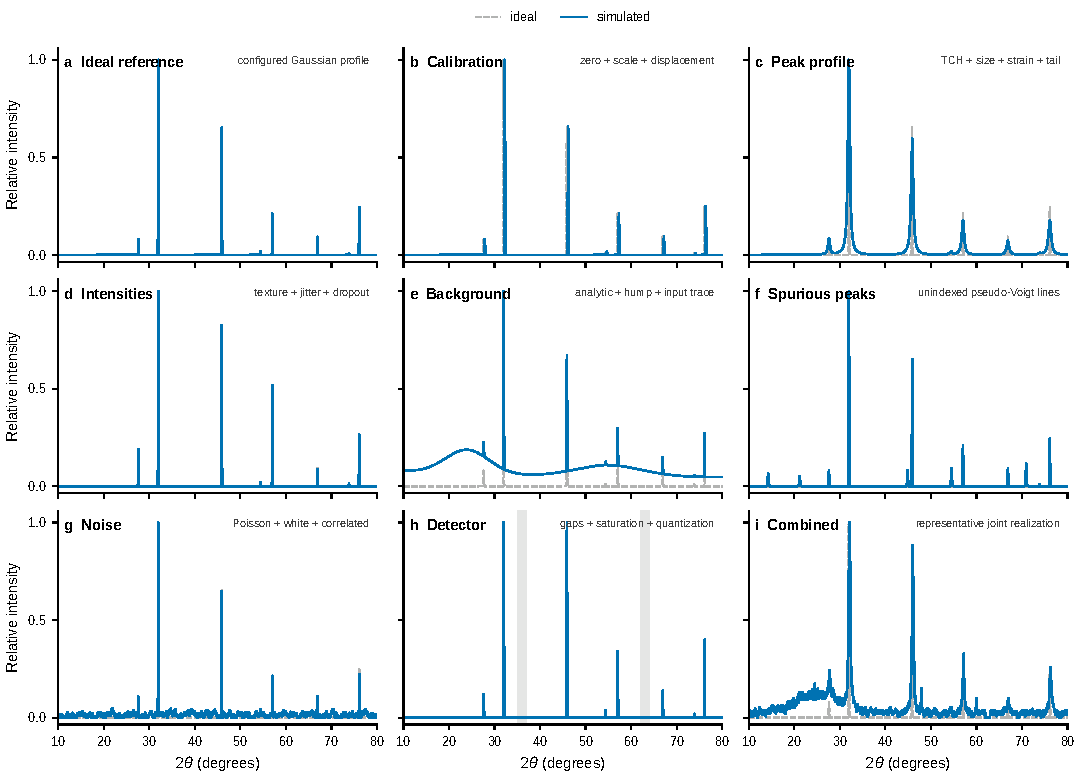
\includegraphics[width=\textwidth]{figures/artifact_gallery.pdf}
  \caption{Configurable experimental effects applied to the same NaCl
  Cu K$\alpha_1$ pattern. The dashed gray curve is the ideal reference and the
  blue curve is the simulated result. Panels isolate (a) the ideal configured
  Gaussian profile, (b) axis calibration and specimen displacement, (c)
  angle-, size-, and strain-dependent peak shape, (d) preferred orientation and
  reflection-wise intensity changes, (e) analytical, amorphous, and
  imported-trace backgrounds, (f) unindexed peaks, (g) counting, independent,
  and correlated noise, and (h) detector gaps, saturation, and quantization.
  Panel (i) combines all effect families. Shaded intervals in (h) mark
  configured detector gaps. Curves are normalized independently for shape
  comparison.}
  \label{fig:artifacts}
\end{figure}

An executable
\href{https://github.com/FrederikLizakJohansen/BraggCalculator/blob/main/notebooks/artifact_simulation.ipynb}{CIF-to-pattern notebook}
follows the same workflow from structure loading through individual component
construction, \texttt{.xye} background import, combined simulation,
visualization, and an exact seed-reproducibility check.

\section{Validation and performance}

Correctness is assessed at three levels: analytical unit tests, extinction and
occupancy cases, and comparisons of X-ray and neutron line patterns with
pymatgen as an implementation reference. The constructed examples in
Figure~\ref{fig:oracle} cover NaCl, SrTiO$_3$, and a triclinic SiO$_2$ cell.
Across 172 X-ray powder lines, the largest position difference is
$4.3\times10^{-14}$ degrees and the largest normalized-intensity difference is
$3.6\times10^{-14}$ percentage points. Applying the same area-normalized
Gaussian independently to both line patterns gives maximum pointwise profile
differences of $1.1\times10^{-11}$ and $2.1\times10^{-12}$ percentage points at
full widths at half maximum of 0.1 and 0.5 degrees, respectively. These values
remain far below the validation tolerances, and the stronger peak overlap does
not conceal a line-pattern discrepancy.

\begin{figure}[htbp]
  \centering
  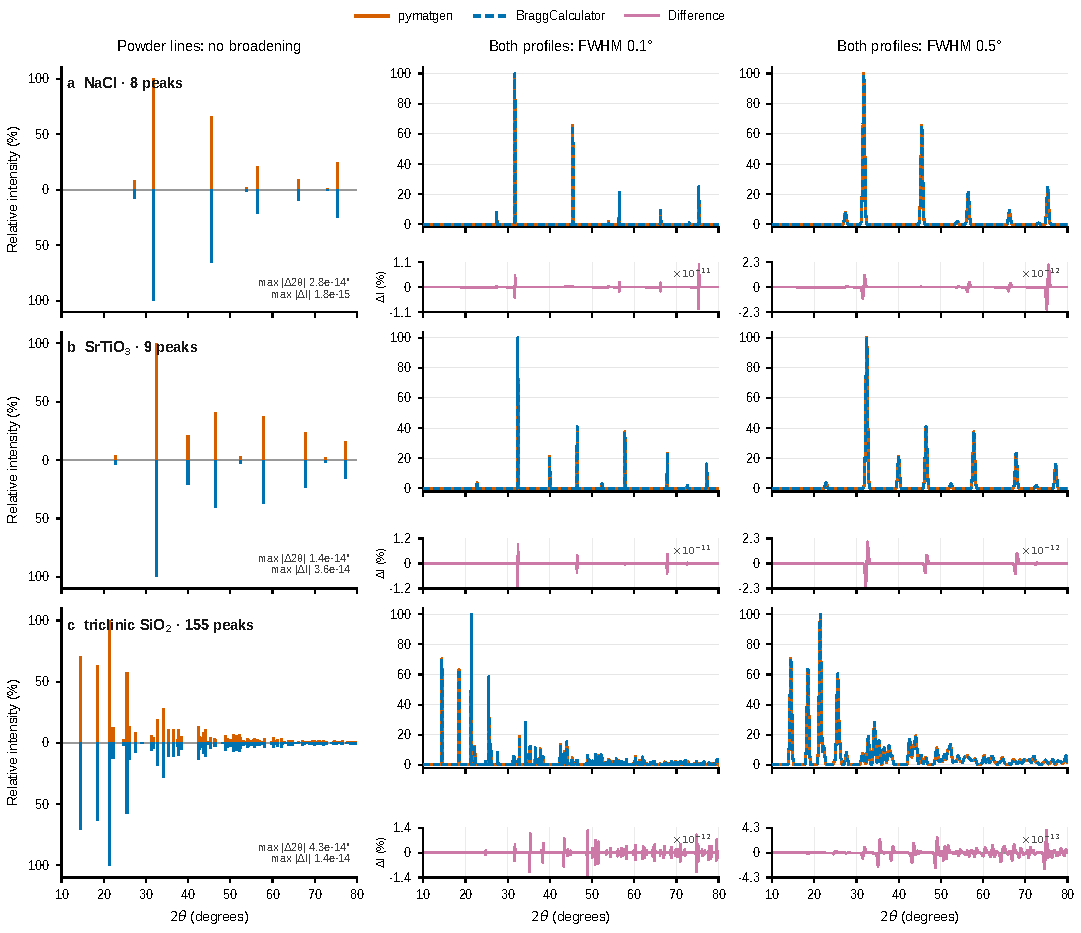
\includegraphics[width=\textwidth]{figures/pattern_comparison_xray.pdf}
  \caption{Oracle comparison before broadening (left) and after applying the
  same area-normalized Gaussian to both implementations at 0.1 degrees
  (centre) and 0.5 degrees (right) full width at half maximum. Orange pymatgen
  and dashed blue BraggCalculator profiles are overlaid; the magenta lower
  trace is their pointwise BraggCalculator-minus-pymatgen difference on the
  displayed scientific scale.}
  \label{fig:oracle}
\end{figure}

A frozen corpus test, summarized in Figure~\ref{fig:cif-validation}, broadens
this implementation comparison beyond constructed examples. Seventy CIF
records from the Crystallography Open Database \citep{grazulis2009} were
selected before comparison, with ten structures from each crystal system, 62
declared space groups, 3--992 supplied sites, and 31 disordered structures. COD
releases its data under CC0 \citep{cod2026}. The corpus records every COD
revision and file hash. Across 57,693 X-ray and 58,819
neutron powder lines, all 140 structure--radiation
comparisons pass. The largest line-position difference is
$7.1\times10^{-14}$ degrees and the largest normalized-intensity difference is
$7.5\times10^{-13}$ percentage points. Both implementations receive the same
pymatgen-parsed structure, which isolates the diffraction calculation from
parser differences; parser warnings remain recorded in the result artifact.
The comparison therefore establishes implementation agreement, not
experimental validation of the deposited structures or the kinematic model.

\begin{figure}[htbp]
  \centering
  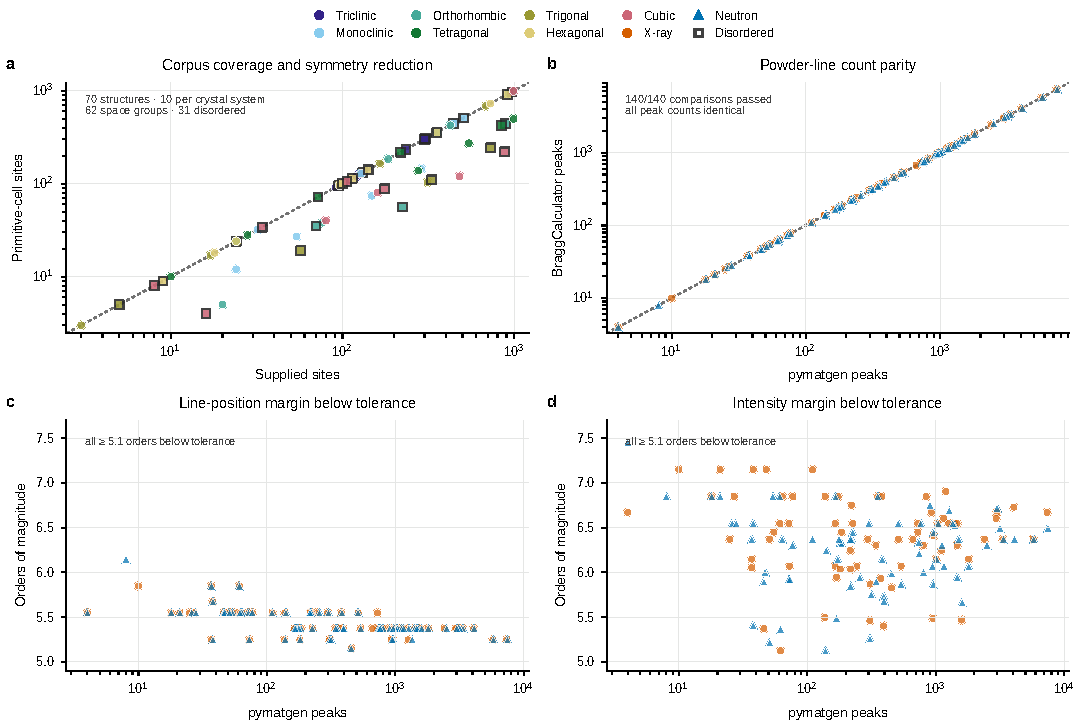
\includegraphics[width=\textwidth]{figures/cif_validation_summary.pdf}
  \caption{Frozen COD corpus coverage and pymatgen agreement. (a) Supplied and
  primitive-cell sites for 70 structures; color denotes crystal system,
  squares denote disorder, and the dashed line is equality. (b)
  BraggCalculator and pymatgen powder-line counts for X-ray circles and neutron
  triangles; all 140 comparisons lie on equality. (c,d) Maximum line-position
  and normalized-intensity errors expressed as orders of magnitude below their
  respective acceptance tolerances. Every comparison has at least a 5.1-order
  margin.}
  \label{fig:cif-validation}
\end{figure}

To complement repeated measurements on constructed scaling cases, a one-pass
throughput benchmark measures the complete heterogeneous corpus after CIF
parsing. Each structure is evaluated exactly once per radiation mode and
implementation, giving 140 distinct calculations per execution path; the
implementation order alternates between successive timings, and every timed
output passes the line-pattern comparison. NumPy CPU completes the corpus in
20.64 s versus 94.75 s for its same-record pymatgen reference, a 4.59-fold
speedup. PyTorch CPU takes 19.08 s versus 94.88 s (4.97-fold), while PyTorch
CUDA takes 7.37 s versus 97.09 s (13.17-fold). The matched PyTorch totals give
a 2.59-fold direct CUDA acceleration. CUDA is faster than PyTorch CPU for 74 of
140 individual calculations; its larger gains on the more expensive structures
therefore dominate the summed runtime despite overhead on smaller cases
(Figure~\ref{fig:cod-throughput}).

\begin{figure}[htbp]
  \centering
  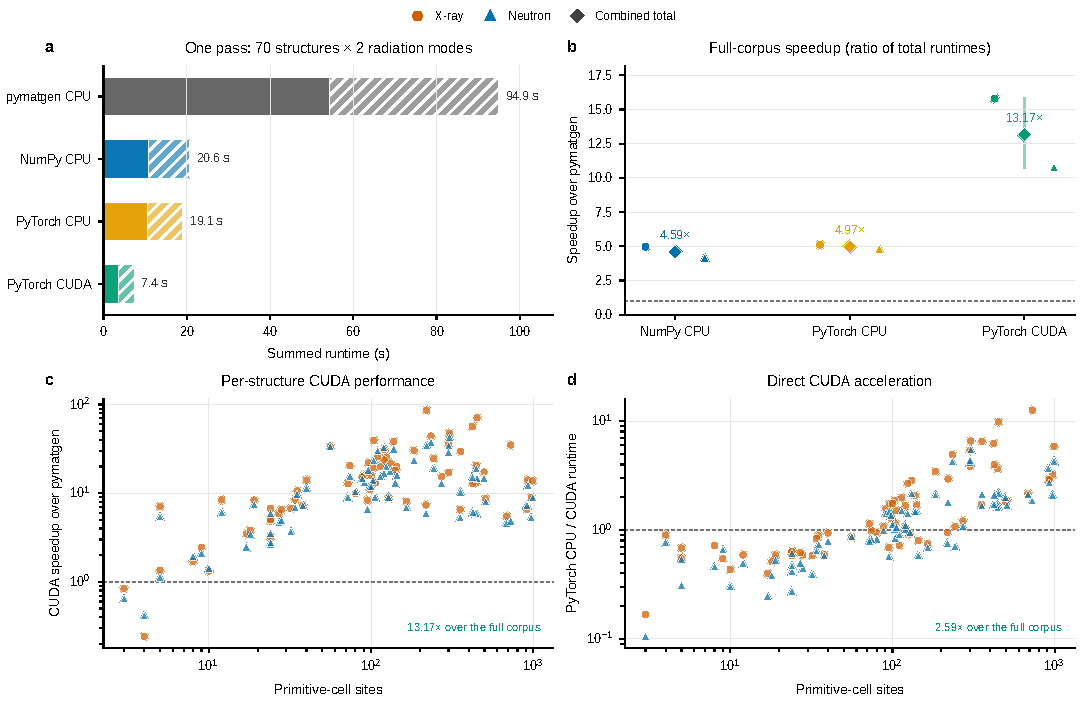
\includegraphics[width=\textwidth]{figures/cod_throughput.pdf}
  \caption{One-pass throughput on the frozen COD corpus after CIF parsing. (a)
  Summed runtime for 70 X-ray and 70 neutron calculations; unhatched and
  hatched segments denote the two modes, and the pymatgen bar uses the median
  per-mode totals from the three matched records. (b) Same-record
  pymatgen-to-BraggCalculator ratios for X-ray circles, neutron triangles, and
  the combined-total diamonds. (c) Per-structure CUDA speedup over pymatgen.
  (d) Direct matched PyTorch CPU-to-CUDA runtime ratio, where values above one
  favor CUDA. Points in (c,d) are single distinct structure--radiation
  calculations; aggregate ratios use summed runtimes across the full corpus.}
  \label{fig:cod-throughput}
\end{figure}

The controlled scaling benchmark validates every case before timing.
Figure~\ref{fig:scaling} reports seven interleaved repeats for NumPy CPU,
PyTorch CPU, and float64 PyTorch CUDA execution on one WSL2 host with an NVIDIA
RTX A3000 Laptop GPU. The three records use the same revision, dependencies,
cases, thread limits, and timing protocol. ``Supplied sites'' counts the sites
in the structure passed to both calculators, before primitive-cell reduction.
For P1 cells containing 4--256 irreducible sites, the NumPy cached speedup over
pymatgen is 18.7--49.3 times and its end-to-end speedup is 13.5--20.0 times. The
CUDA run becomes increasingly effective as the reflection-by-site workload
grows. It crosses the matched PyTorch CPU runtime at 64 sites and is 8.7 times
faster cached and 6.5 times faster end-to-end at 256 sites; its corresponding
speedups over host pymatgen are 190 and 132 times.

For NaCl supercells containing 8--512 supplied sites,
\texttt{BraggCalculator} reduces every case to the same two-site primitive cell
and 410 reciprocal-lattice points. The GPU workload therefore remains fixed as
the supplied supercell grows, leaving the CUDA calculation dominated by launch,
transfer, and synchronization overhead. Against the matched PyTorch CPU run,
CUDA is
5.2--5.7 times slower cached and 1.4--1.5 times slower end-to-end across these
four cases. The CUDA end-to-end speedup over host pymatgen nevertheless rises
from 0.81 to 77.1 times; this increase comes from primitive-cell reduction, not
from a growing GPU workload. Each plotted speedup uses the pymatgen samples in
the same timing record, while the direct device row compares the matched
PyTorch CPU and CUDA records.

\begin{figure}[htbp]
  \centering
  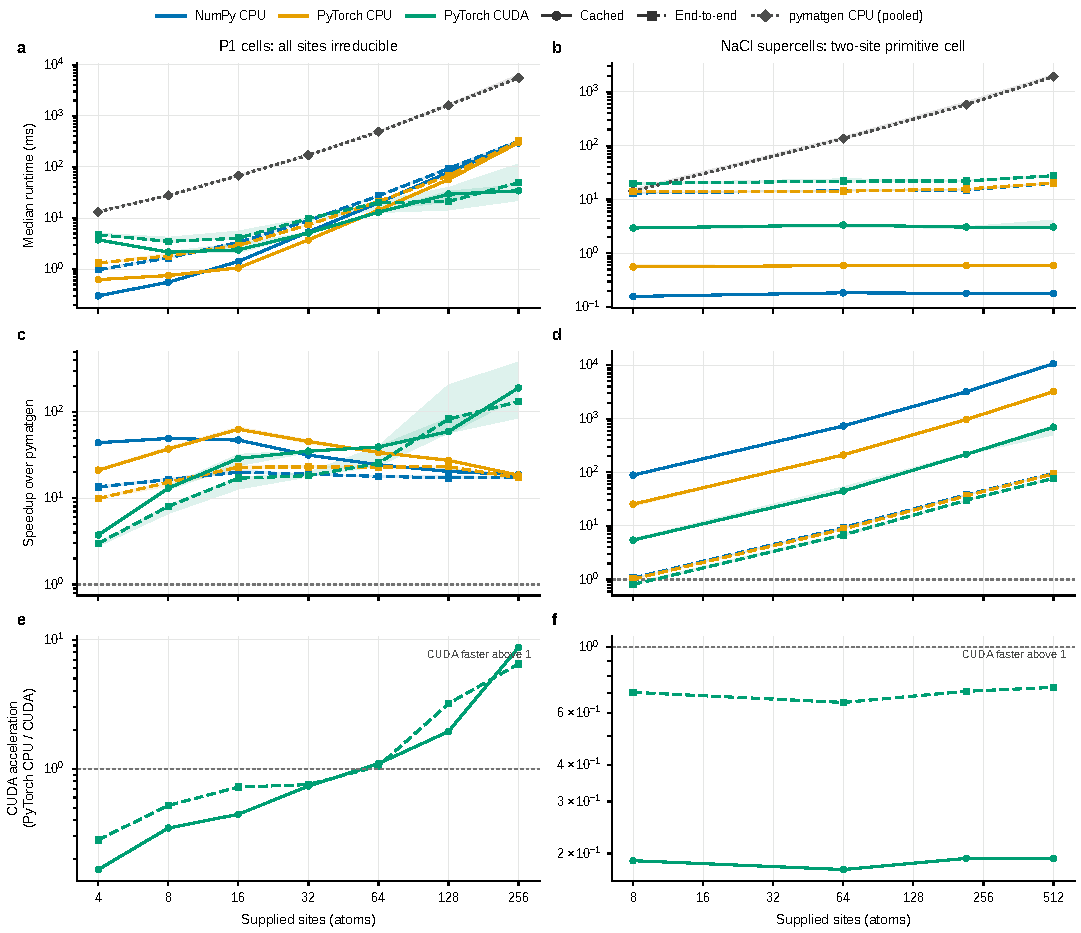
\includegraphics[width=\textwidth]{figures/scaling_speedup.pdf}
  \caption{Runtime, speedup over pymatgen, and direct CUDA acceleration for
  increasing irreducible P1 cells (left) and symmetry-reducible NaCl
  supercells (right). Color identifies the BraggCalculator execution path;
  circles with solid lines are cached timings and squares with dashed lines are
  end-to-end timings. Runtime lines show medians and speedup lines show ratios
  of medians; bands show interquartile ranges over the raw timings or paired
  speedup ratios. The gray pymatgen runtime pools the three same-host records,
  while each speedup uses the pymatgen repeats in its own timing record. The
  bottom row is the ratio of the PyTorch CPU and CUDA median runtimes, so values
  above one indicate a CUDA advantage. Cached timings reuse symmetry analysis
  and the prepared reflection set; end-to-end timings include all
  preprocessing.}
  \label{fig:scaling}
\end{figure}

\section{Research impact statement}

\texttt{BraggCalculator} makes the same validated periodic diffraction model
available through NumPy arrays and differentiable PyTorch tensors. The
repository includes the structure generators, implementation comparisons, raw
timing samples, figure scripts used above, and an executable CIF-to-pattern
artifact tutorial. Continuous
integration covers two Python versions, both diffraction modes, general and
disordered structures, automatic differentiation, experimental-effect
components, and the public result objects. A small public API, Apache-2.0
license, typed package marker, pymatgen and optional ASE inputs, and
NumPy/PyTorch backends support reuse in established Python materials workflows.
The differentiable path enables gradient-based fitting and machine-learning
applications without reimplementing the diffraction equations in a tensor
framework, while the optional effects support reproducible synthetic training
and robustness datasets.

\section{Acknowledgements}

The author thanks the maintainers of pymatgen and spglib for their open
crystallographic software and data resources.

\bibliographystyle{plainnat}
\bibliography{paper}

\end{document}
